\paragraph{\distrib{Ubuntu/Kubuntu}}
\label{Ubuntu:IP}
Il existe deux manières de configurer tes paramètres réseaux: l'une utilise les outils graphiques de l'environnement que tu as choisi (Gnome ou KDE), l'autre utilise simplement la ligne de commande. Bien sûr, les outils graphiques ne sont qu'un intermédiaire modifiant les fichiers dont on te parle plus bas. Ils te permettent parfois d'enregistrer une configuration réseau, ce qui facilite la gestion si tu rentres souvent chez toi.

\begin{description}
\item[Configuration à l'aide des outils graphiques]
Tu peux modifier tes paramètres réseau \emph{via} l'icône présente dans ta barre des tâches symbolisant le réseau: c'est un raccourci vers \app{KNetworkManager} sous Kubuntu (KDE; l'icône représente un c\^able réseau) et vers \app{l'applet réseau} sous Ubuntu (Gnome; l'icône en haut à droite symbolisant un réseau, menu \menu{Propriétés}).

Un simple clic droit dessus affiche un menu te permettant d'ouvrir la fenêtre de configuration. \emph{Attention}, ici le réseau est à configurer en \emph{statique}; pas en automatique avec DHCP ! Rentre ensuite ton adresse IP, ta passerelle, ton adresse de \emph{broadcast} et ton masque de sous-réseau.

Ensuite il faut configurer la résolution DNS, sous Kubuntu va sur l'onglet \menu{Système de noms de domaines} ou dans l'outil de configuration du réseau
(\menu{Paramètres du système}, \menu{Réseau}). Les adresses IP des serveurs DNS sont les suivantes: \server{129.104.201.53} et \server{129.104\-.201.51}, le domaine réseau
est \server{eleves.polytechnique.fr}, tu peux aussi ajouter \server{polytechnique.fr} pour accéder plus facilement aux machines des salles info. Choisis un nom de machine
(en général ton pseudo) que tu reporteras dans \app{qRezix} pour qu'il soit enregistré.


%\imagepos{images/kubuntu_config_reseau0}{0.65}{Configuration du réseau sous Kubuntu}{!ht}
%\imagepos{images/kubuntu_config_reseau1}{0.55}{Configuration de la résolution DNS sous Kubuntu}{!ht}

\noindent
  \begin{figure*}[!h]
    \begin{center}  
      \subfloat[Configuration IP]{ 
      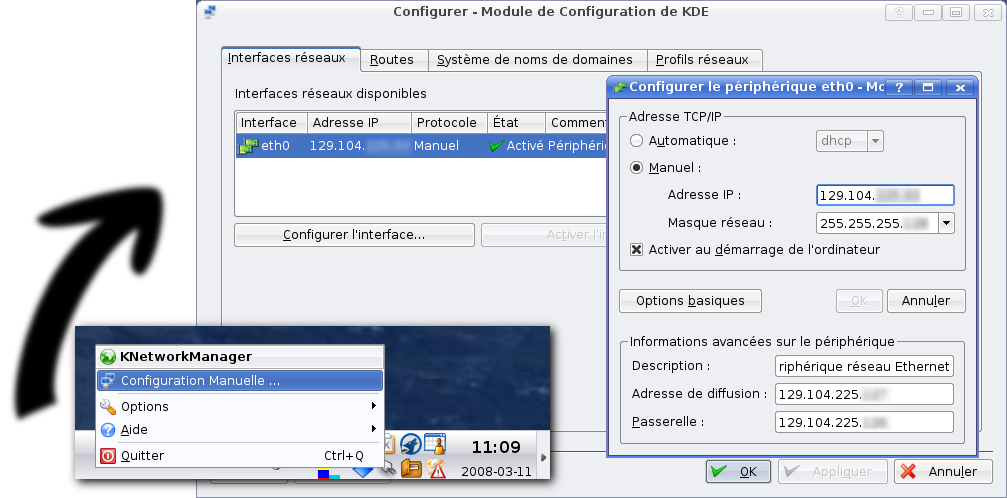
\includegraphics[width=0.65\textwidth]{images/kubuntu_config_reseau0}} \\
%      \hspace{\stretch{1}}
      \subfloat[Configuration DNS]{ 
	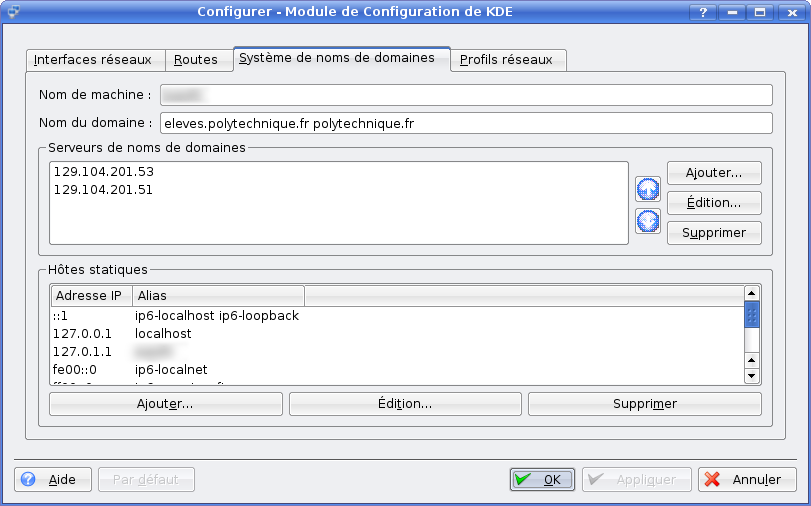
\includegraphics[width=0.65 \textwidth]{images/kubuntu_config_reseau1}}
         	 \caption{Configuration réseau}
    \end{center}
  \end{figure*}
  
%%%%%%%%%%%%%%%%%%%%%%%%%%%%%%%%%%%%%%%%%%%%%%%%%%%%%%%%%%%%%%%%%%%%%%%%%%%%%%%%%%%%%%%%%%%%%%%%%%%%%%%%%%%%%%%%%%%%%%%%%%%%%%
%%%%%%%%%%%%%%%%%%%%%%%%%%%%%%%%%%%%%%%%%%%%%%%%%%%%%%%%%%%%%%%%%%%%%%%%%%%%%%%%%%%%%%%%%%%%%%%%%%%%%%%%%%%%%%%%%%%%%%%%%%%%%%
%%%%%%%%%%%%%%%%%%%%%%%%%%%%%%%%%%%%%%%%%%%%%%%%%%%%%%%%%%%%%%%%%%%%%%%%%%%%%%%%%%%%%%%%%%%%%%%%%%%%%%%%%%%%%%%%%%%%%%%%%%%%%%

\item[Configuration en ligne de commande]
 Tu peux également modifier directement les fichiers de configuration réseau comme indiqué ci-dessous avec ton éditeur de texte préféré (\app{vim}, \app{emacs}, \dots), le tout avec les droits
 administrateur évidemment! Encore une fois,  les étapes qui suivent peuvent \^etres entièrement réalisées avec les outils graphiques mentionnés plus haut.

 \begin{itemize}
 \item Le fichier \file{/etc/hostname} contient ton nom de machine. Il doit contenir uniquement: 
 \cmdline[0.85]{tonPseudo.eleves.polytechnique.fr}
  
 \item Le fichier \file{/etc/resolv.conf} décrit comment associer le nom d'une machine à une adresse IP.
 Il doit contenir: 
 \cmdline[0.85]{
 domain eleves.polytechnique.fr\\
 search eleves.polytechnique.fr polytechnique.fr\\
 nameserver 129.104.201.53\\
 nameserver 129.104.201.51
 }
 
 \item Le fichier \file{/etc/network/interfaces} contient entre autres ton adresse IP,
 ton sous-réseau et la passerelle pour en sortir. Ce fichier doit
 ressembler (avec éventuellement une configuration wifi à la suite\ldots,
 voir page~\pageref{wifi}) à :
  \cmdline[0.85]{
 \# The loopback network interface\\
 auto lo\\
 iface lo inet loopback\\
 \\
 \# The primary network interface\\
 auto eth0\\
 iface eth0 inet static\\
         address   129.104.AAA.BBB\\
         netmask   255.255.FFF.DDD\\
         broadcast 129.104.GGG.EEE\\
         gateway   129.104.GGG.CCC
 }
 
 \end{itemize}
 
 Ensuite il faut redémarrer ta configuration réseau (les outils graphiques devraient le faire tout seuls après validation) :
 
 \cmdline{\$ sudo /etc/init.d/networking restart}
 
 \end{description}
%%%%%%%%%%%%%%%%%%%%%%%%%%%%%%%%%%%%%%%%%%%%%%%%%%%%%%%%%%%%%%%%%%%%%%%%%%%%%%%%%%%%%%%%%%%%%%%%%%%%%%%%%%%%%%%%%%%%%%%%%%%%%%
%%%%%%%%%%%%%%%%%%%%%%%%%%%%%%%%%%%%%%%%%%%%%%%%%%%%%%%%%%%%%%%%%%%%%%%%%%%%%%%%%%%%%%%%%%%%%%%%%%%%%%%%%%%%%%%%%%%%%%%%%%%%%
%%%%%%%%%%%%%%%%%%%%%%%%%%%%%%%%%%%%%%%%%%%%%%%%%%%%%%%%%%%%%%%%%%%%%%%%%%%%%%%%%%%%%%%%%%%%%%%%%%%%%%%%%%%%%%%%%%%%%%%%%%%%%%

Une fois ta configuration réseau terminée, tu peux la tester en \emph{pinguant} \fkz (dans une console), où tu devrais voir quelque chose comme :

\cmdline{\$ ping frankiz\\
PING frankiz.eleves.polytechnique.fr (129.104.201.51) 56(84) bytes of data.\\
64 bytes from Frankiz.eleves.polytechnique.fr ...}

 \subparagraph{Configuration du gestionnaire de paquets} \label{ubuntu_mirror} Il faut désormais configurer le gestionnaire de paquets pour
qu'il utilise les miroirs du BR et non les miroirs à l'extérieur du
campus, qui sont plus lents.

Le fichier \file{/etc/apt/sources.list} liste les miroirs utilisés par le gestionnaire de paquets. Il faut commenter la première ligne (qui
correspond au CD d'installation) ainsi que toutes les lignes non commentées du fichier (qui correspondent aux miroirs extérieurs au campus) de la
façon suivante:
\cmdline{deb cdrom:[...]/ version main restricted}
devient
\cmdline{\#deb cdrom:[...]/ version main restricted}

Il faut ensuite ajouter les lignes suivantes, qui correspondent aux miroirs du BR, au \emph{début} du fichier:
\cmdline{
deb ftp://miroir/ubuntu version main restricted universe multiverse\\
deb ftp://miroir/ubuntu version-updates main restricted universe multiverse\\
deb ftp://miroir/ubuntu version-security main restricted universe multiverse
}
où \textbf{version} correspond à la version d'Ubuntu installée sur ton ordinateur. La version actuelle est \textbf{intrepid} et la précédente est \textbf{hardy}.

Tu peux aussi utiliser le dépôt suivant mais attention il contient des logiciels \emph{non supportés par l'équipe de développement d'Ubuntu} (en particulier il peut arriver que certains logiciels contiennent des erreurs):
\cmdline{deb ftp://miroir/ubuntu [version]-backports main restricted universe multiverse}

Le BLL (Binet Logiciels Libres) dispose par ailleurs d'un miroir non-officiel qui contient \app{qRezix} ainsi que des paquets très importants (codecs
vidéo, java,\dots) ou pas (\app{bureau 3D}, \app{Google Earth}, \dots), non inclus dans la distribution de base pour diverses raisons, en particulier légales ou
éthiques. Pour en profiter, il faut rajouter à la suite des lignes précédentes:
\cmdline{deb ftp://miroir/bll [version] main}


On finit par vérifier que tout fonctionne en mettant à jour la liste
des paquets disponibles:
\cmdline{\$ sudo aptitude update}

S'il n'y a pas de message d'erreur c'est que tout fonctionne bien.

\textbf{NB:} on peut aussi faire cette configuration depuis \app{synaptic} (ubuntu) ou \app{adept} (kubuntu), il suffit d'aller dans le menu faisant référence aux dépôts.
